\documentclass[a4paper,12pt]{article}

% don't forget the document class, generally : \documentclass[a4paper,12pt]{article}

\usepackage[utf8]{inputenc}
\usepackage[french]{babel}
\usepackage{graphicx}
\usepackage{gensymb}
\usepackage{amsmath}
\usepackage{float}
\usepackage{scrextend}
\usepackage{caption} 
\usepackage{siunitx}
\usepackage{enumitem}
\usepackage{amsthm}
\usepackage{fancyhdr}
\usepackage{amssymb}
\usepackage{wrapfig}
\usepackage{geometry}
\usepackage{standalone}
\usepackage{import}
\usepackage[usenames, dvipsnames]{color}

 \usepackage{biblatex} % manages bibliography and references
\addbibresource{sample.bib}


\geometry{hmargin=1in, vmargin=1in}

 \newenvironment{absolutelynopagebreak}
 {\par\nobreak\vfil\penalty0\vfilneg
 \vtop\bgroup}
 {\par\xdef\tpd{\the\prevdepth}\egroup
 \prevdepth=\tpd}
 
 \pagestyle{fancy}                        
\fancyhf{}                               
\fancyhf[HL]{Application des maths}                
\fancyhf[HR]{Géométrie euclidienne}             
\fancyhf[FC]{\thepage/\pageref{Lastpage}}
 
\newtheorem{definition}{Définition}[section]
\newtheorem{theorem}{Théorème}
\newtheorem{corollary}{Corollaire}[theorem]
\newtheorem{lemma}[theorem]{Lemme}
\newtheorem*{hyp}{Hypothèse}
\newtheorem*{concl}{Conclusion}
\newtheorem*{remark}{Remarque}

\captionsetup{format=default,labelformat=simple,labelsep=colon,
justification=justified,font={sf,small},labelfont=bf,
textfont=default} 



\begin{document}

\subsubsection{Premier cas de similitude}
\begin{theorem}
Deux triangles dont les angles sont respectivement isométriques sont semblables.
\end{theorem}

\begin{remark}
Si deux triangles ont deux angles respectivement isométriques, leur dernier angle est aussi isométrique, car la somme des angles d'un triangle est une constante (théorème \ref{th:180}). Imaginons $\triangle ABC$ et $\triangle A'B'C'$. Si nous considérons $\alpha \equiv \alpha'$ et $\beta \equiv \beta'$, alors $\alpha + \beta = 180 - \gamma$ et $\alpha' + \beta' = 180 - \gamma'$, donc $\gamma \equiv \gamma'$.

\end{remark}


\begin{proof}
Nous considérons deux triangles $\triangle ABC$ et $\triangle A'B'C'$.

\begin{figure}[H]
        \centering
        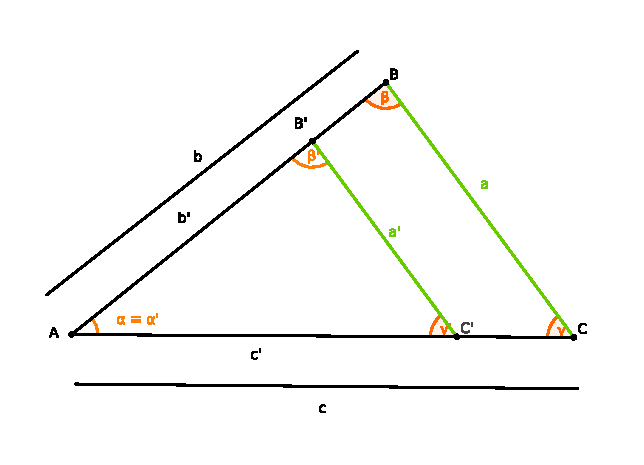
\includegraphics[scale=0.2]{similitude1.1.eps}
    \end{figure}

\begin{hyp}
$\alpha \equiv \alpha'$ et $\beta \equiv \beta'$
\end{hyp}

\begin{concl}
$\frac{a}{a'} = \frac{b}{b'} = \frac{c}{c'}$
\end{concl}

Nous commençons par faire coïncider $\alpha$ et $\alpha '$.\\

\begin{figure}[H]
        \centering
        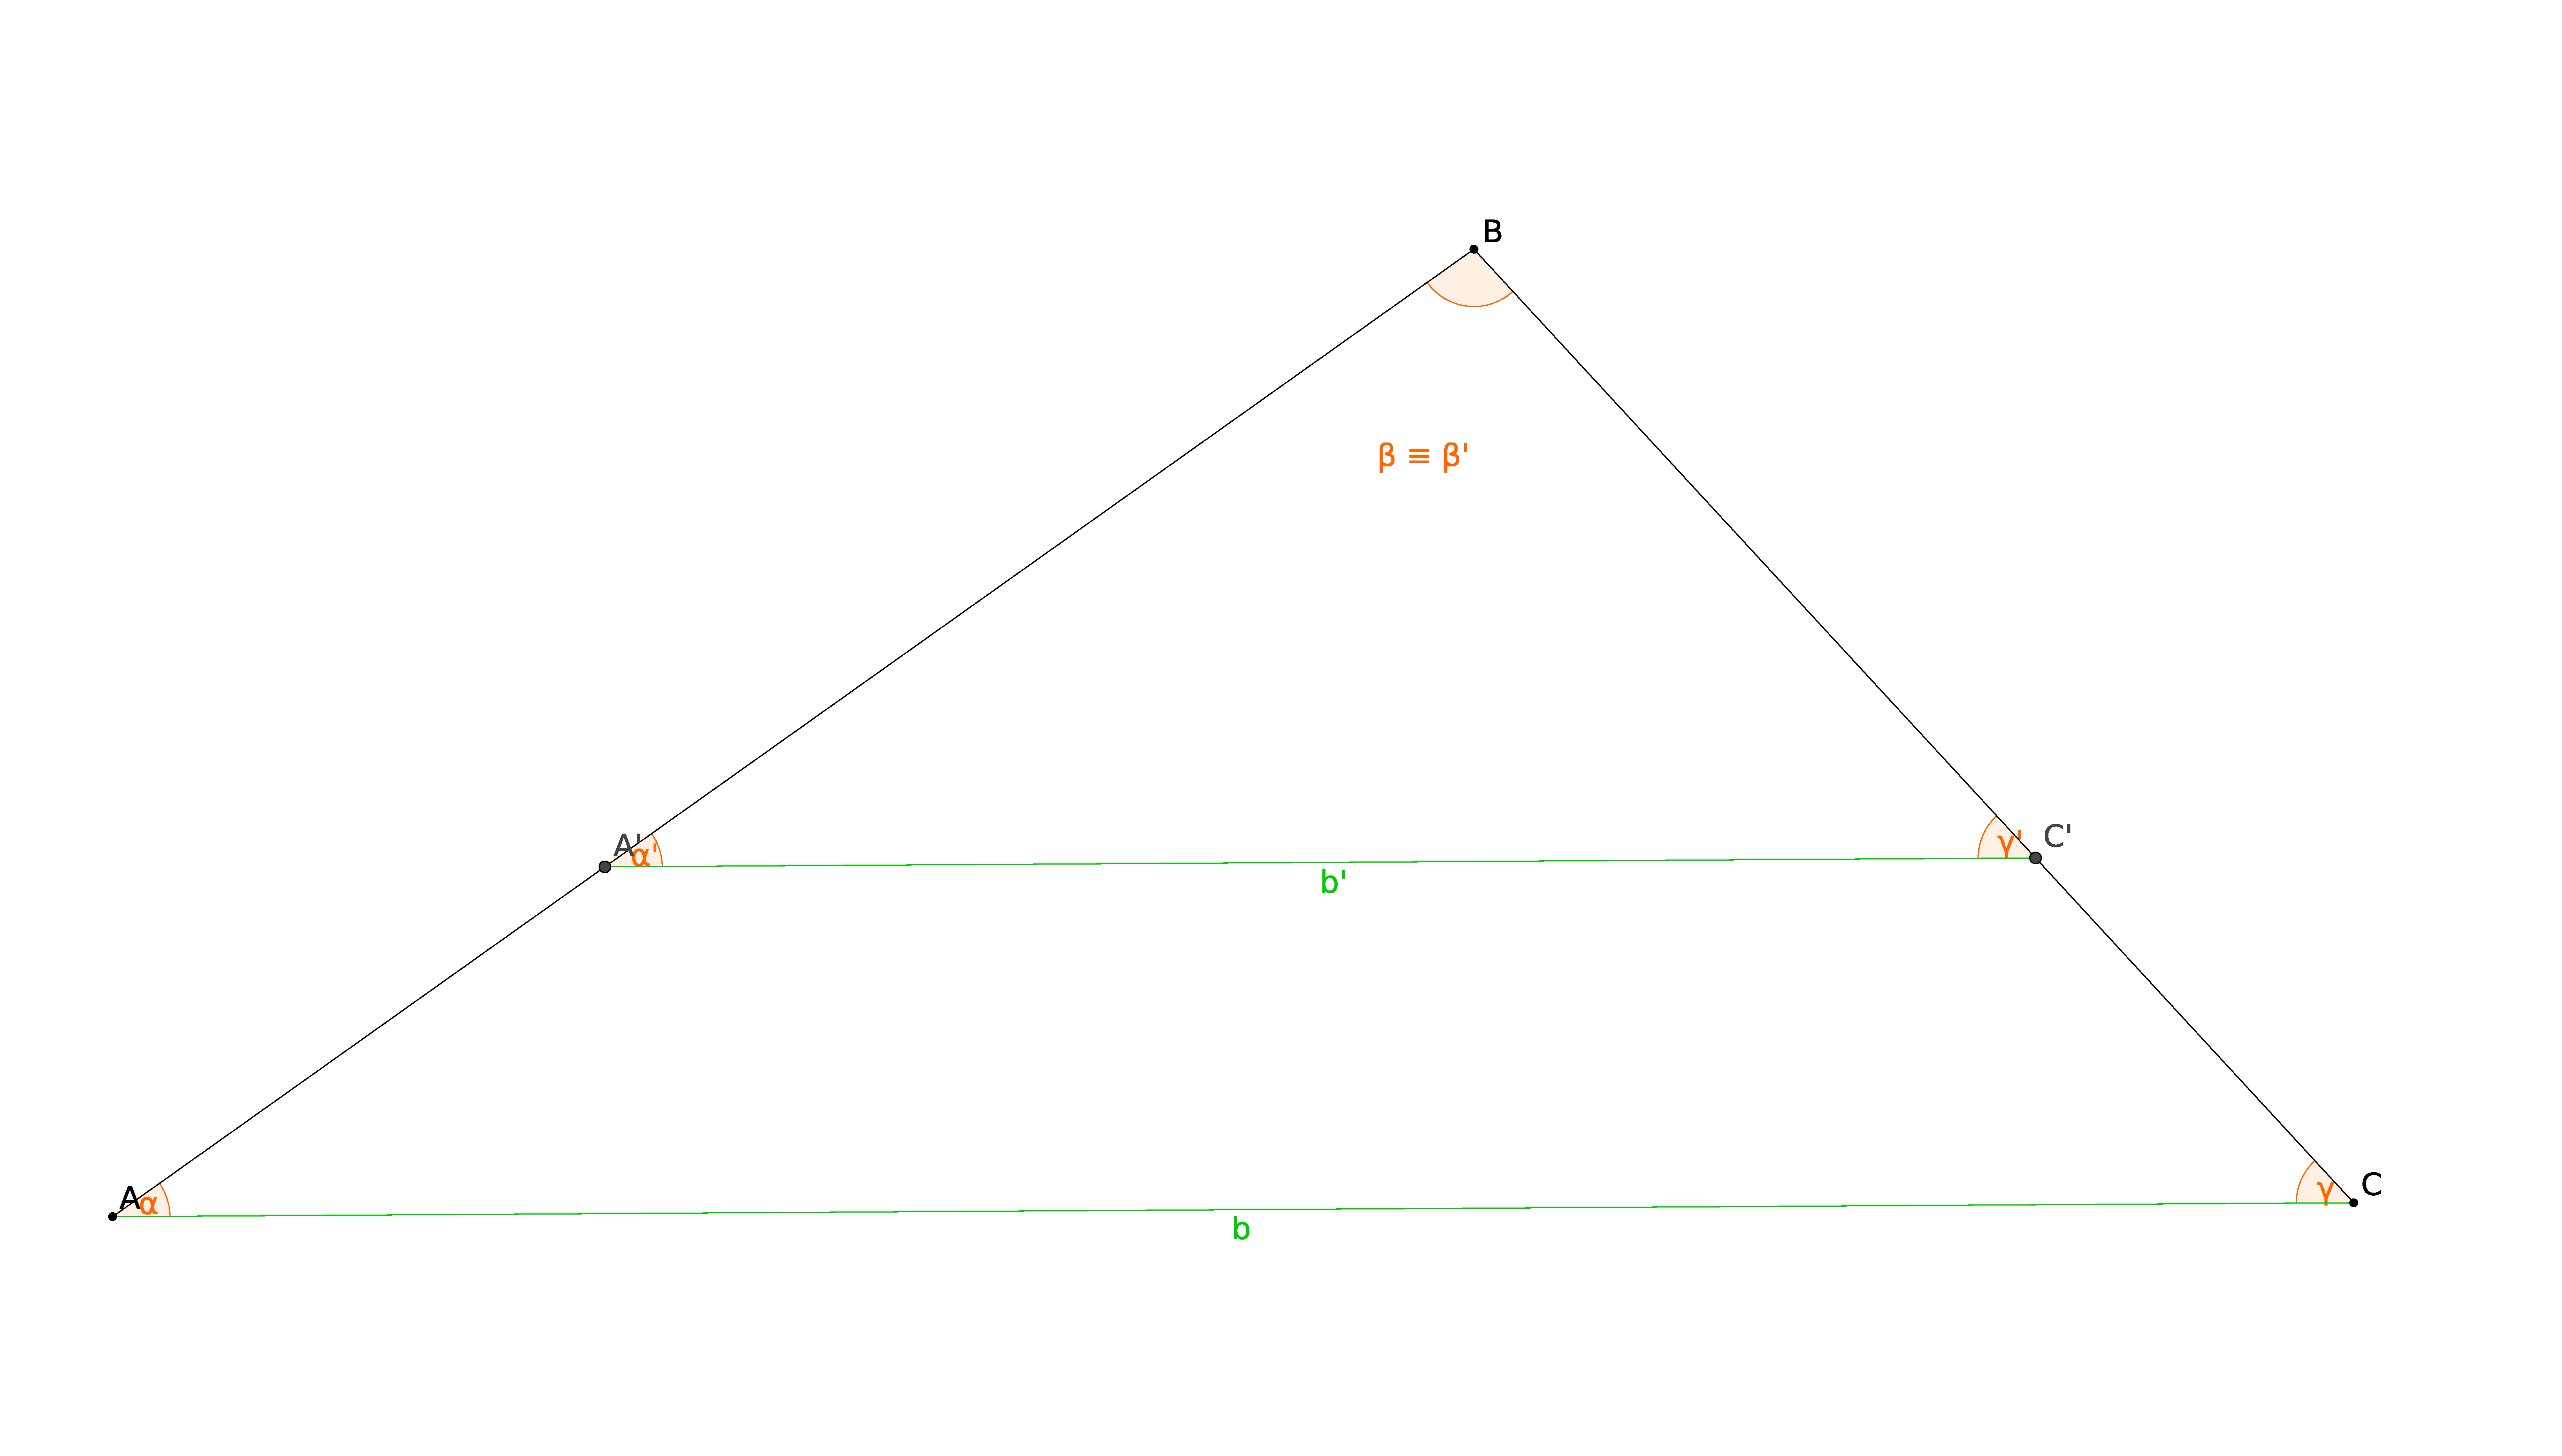
\includegraphics[scale=0.2]{similitude1.2.eps}
    \end{figure}

Puisque $\beta \equiv \beta '$ et $\gamma \equiv \gamma '$, on observe que $a \parallel a'$ grâce au théorème de la transversale.
Ainsi, si l'on imagine une droite parallèle à $a$ et $a'$ et passant par $A$, on observe que $\frac{b'}{b} = \frac{c'}{c}$.\\
Si l'on répète cette opération en faisant coïncider $\beta$ et $\beta '$, l'on obtient que $\frac{a'}{a} = \frac{c'}{c}$.

\begin{figure}[H]
        \centering
        \includegraphics[scale=0.2]{similitude1.3.eps}
    \end{figure}
Par conséquent, $\frac{a'}{a} = \frac{b'}{b} = \frac{c'}{c}$.


\end{proof}
\end{document}